% generated by scripts/pkl_to_latex.py
% source PKL : vscan_v1_L6_Ne6_U10_t1_mode-uniform_nmin2_solver-gcg_full_es_restarts8_iter300_kmax8_tol1em09_V0to15_N16-2f7c06936fa2.pkl
% scan type  : vscan
% state      : ex_singlet
% requires   : \usepackage{pgfplots} \pgfplotsset{compat=1.18}
% colours match the matplotlib PDF (tab10 cycle)
\definecolor{gmeC0}{HTML}{1F77B4}
\definecolor{gmeC1}{HTML}{FF7F0E}
\definecolor{gmeC2}{HTML}{2CA02C}
\definecolor{gmeC3}{HTML}{D62728}
\definecolor{gmeC4}{HTML}{9467BD}
\definecolor{gmeC5}{HTML}{8C564B}
\definecolor{gmeC6}{HTML}{E377C2}
\definecolor{gmeC7}{HTML}{17BECF}

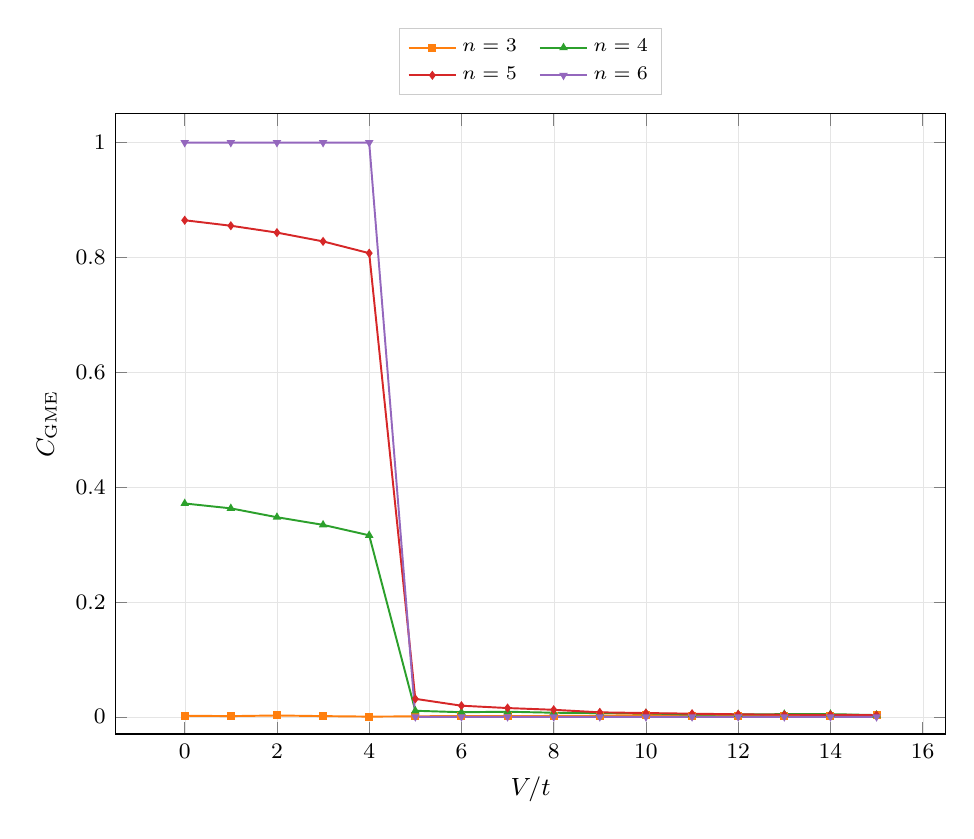
\begin{tikzpicture}
  \begin{axis}[
    width=\columnwidth,
    height=0.78\columnwidth,
    xlabel={$V/t$},
    ylabel={$C_{\mathrm{GME}}$},
    grid=both,
    grid style={line width=.1pt, draw=gray!20},
    tick label style={font=\footnotesize\rmfamily, /pgf/number format/fixed},
    label style={font=\small\rmfamily},
    scaled ticks=false,
    legend style={font=\scriptsize\rmfamily, draw=gray!40, at={(0.5,1.03)}, anchor=south, /tikz/every even column/.append style={column sep=6pt}},
    legend cell align={left},
    legend columns=2,
    ymin=-0.03,
    ymax=1.05,
  ]
    \addplot[color=gmeC1, mark=square*, mark size=1.1pt, line width=0.7pt] coordinates {
        (0,0.001861) (1,0.001193) (2,0.002331) (3,0.001199)
        (4,0.000344) (5,0.000815) (6,0.001489) (7,0.001223)
        (8,0.001531) (9,0.00192) (10,0.003102) (11,0.002111)
        (12,0.001966) (13,0.001243) (14,0.001585) (15,0.002724)
    };
    \addlegendentry{$n=3$}
    \addplot[color=gmeC2, mark=triangle*, mark size=1.1pt, line width=0.7pt] coordinates {
        (0,0.371526) (1,0.363008) (2,0.347555) (3,0.33427)
        (4,0.31606) (5,0.010523) (6,0.00798) (7,0.008834)
        (8,0.007102) (9,0.006413) (10,0.006028) (11,0.003792)
        (12,0.004135) (13,0.004609) (14,0.004647) (15,0.003027)
    };
    \addlegendentry{$n=4$}
    \addplot[color=gmeC3, mark=diamond*, mark size=1.1pt, line width=0.7pt] coordinates {
        (0,0.864713) (1,0.855157) (2,0.843215) (3,0.827884)
        (4,0.807398) (5,0.031276) (6,0.019344) (7,0.015252)
        (8,0.012219) (9,0.007789) (10,0.006558) (11,0.005462)
        (12,0.004355) (13,0.00354) (14,0.003513) (15,0.002861)
    };
    \addlegendentry{$n=5$}
    \addplot[color=gmeC4, mark=triangle*, mark size=1.1pt, mark options={rotate=180}, line width=0.7pt] coordinates {
        (0,1) (1,1) (2,1) (3,1)
        (4,1) (5,0) (6,0) (7,0)
        (8,0) (9,0) (10,0) (11,0)
        (12,0) (13,0) (14,0) (15,0)
    };
    \addlegendentry{$n=6$}
  \end{axis}
\end{tikzpicture}
